\chapter{System Architecture}

\begin{figure}[ht]
 \centerline{\scalebox{1.0}{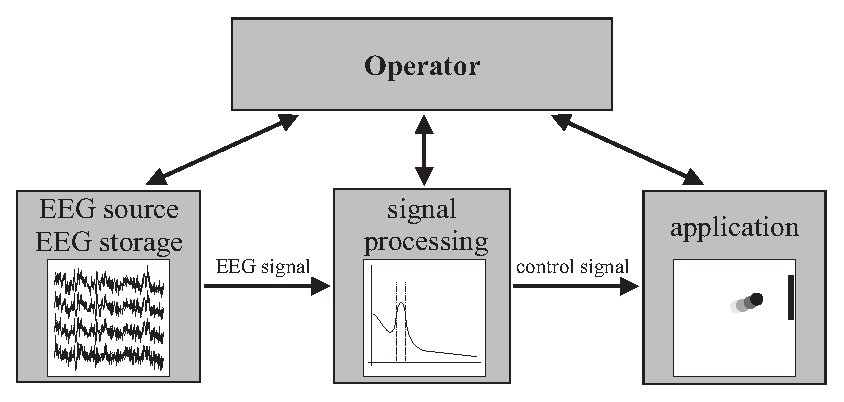
\includegraphics{figures/modules.eps}}}
 \caption{High--level overview of modules in BCI2000}
 \label{mod_overview}
\end{figure}

This partitioning scheme and the used communication protocols are described in 
detail in the BCI2000 Project Outline.


%This section should provide a high-level overview of how the functionality and 
%responsibilities of the system were partitioned and then assigned to subsystems 
%or components. Don't go into too much detail about the individual components 
%themselves (there is a subsequent section for detailed component descriptions). 
%The main purpose here is to gain a general understanding of how and why the 
%system was decomposed, and how the individual parts work together to provide the 
%desired functionality. 

%At the top-most level, describe the major responsibilities that the software 
%must undertake and the various roles that the system (or portions of the system) 
%must play. Describe how the system was broken down into its 
%components/subsystems (identifying each top-level component/subsystem and the 
%roles/responsibilities assigned to it). Describe how the higher-level components 
%collaborate with each other in order to achieve the required results. Don't 
%forget to provide some sort of rationale for choosing this particular 
%decomposition of the system (perhaps discussing other proposed decompositions 
%and why they were rejected). Feel free to make use of design patterns, either in 
%describing parts of the architecture (in pattern format), or for referring to 
%elements of the architecture that employ them. 

%If there are any diagrams, models, flowcharts, documented scenarios or use-cases 
%of the system behavior and/or structure, they may be included here (unless you 
%feel they are complex enough to merit being placed in the Detailed System Design 
%section). Diagrams that describe a particular component or subsystem should be 
%included within the particular subsection that describes that component or 
%subsystem. 

%Note: This section (and its subsections) really applies only to newly developed 
%(or yet-to-be developed) portions of the system. If there are parts of the 
%system that already existed before this development effort began, then you only 
%need to describe the pre-existing parts that the new parts of the system depend 
%upon, and only in enough detail sufficient to describe the relationships and 
%interactions between the old parts and the new parts. Pre-existing parts that 
%are modified or enhanced need to be described only to the extent that is 
%necessary for the reader to gain a sufficient understanding of the nature of the 
%changes that were made. 